\begin{frame}[label=uebersicht]{\only<presentation>{Kursus / Übersicht}}
  \textbf{15.12.2017 : Internettechnologien I, Datenbanktechnologien I}
    \begin{itemize}
      \item IntT I: Dokumentformen, Skriptsprachen, Ajax, responsive Web
      \item DBT I: Datenbanktypen, Technologien, Einstieg SQL
    \end{itemize}
\end{frame}

\section{Internettechnologien I}
\subsection{Dokumentformen}

\only<article>{
  Mit der Entwicklung von http ab 1989 wurde das www begründet und der Austausch von Daten aus Anwendungen heraus zwischen Rechnern ermöglicht. Http wird hauptsächlich benutzt, um mit einem Browser Webseiten zu laden. Dazu fragt der Browser den Server nach einer Seite, der Server liefert sie an den Browser aus, und dieser stellt sie dann dar.

  Bei Webseiten handelt es sich zunächst einmal um mehr oder weniger simple Textdateien. 
}

\begin{frame}{\only<presentation>{Dokumentformen}}
  \begin{itemize}
    \item Warum nicht Word, Pages, \ldots ?
  \end{itemize}
\end{frame}

\only<article>{
  Das Web ist eine unvorstellbar große Sammlung von Dokumenten. Wenn man also im Internet surft, guckt man sich Dokumente an, die auf anderen Rechnern liegen. Nun haben doch alle Word --- warum also ein weiteres Format (html)? Es gibt dazu viele Argumente:
} 

\begin{frame}
  \frametitle{1. Dokumentgrößen}
  \begin{center}
    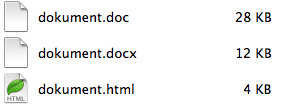
\includegraphics[width=6cm]{pics/Finder.png}
  \end{center}
\end{frame}
%
\begin{frame}
  \frametitle{die Dokumentauszeichnung am Beispiel ``Pages''}
    \begin{center}
      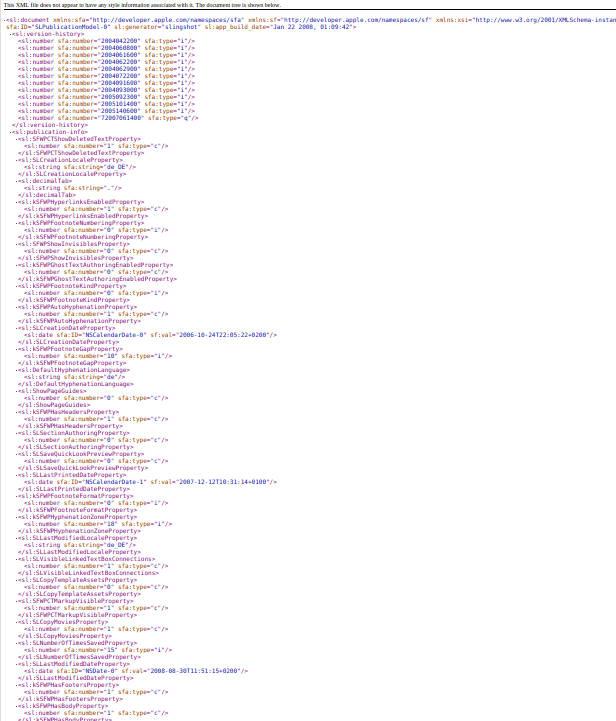
\includegraphics[height=6cm]{pics/auszeichnung.png}
      (noch 12 mal soviel\ldots)
    \end{center}
\end{frame}
%
\begin{frame}{der Dokumentinhalt am Beispiel ``Pages''}
  \framesubtitle{der eigentliche Text}
    \begin{center}
      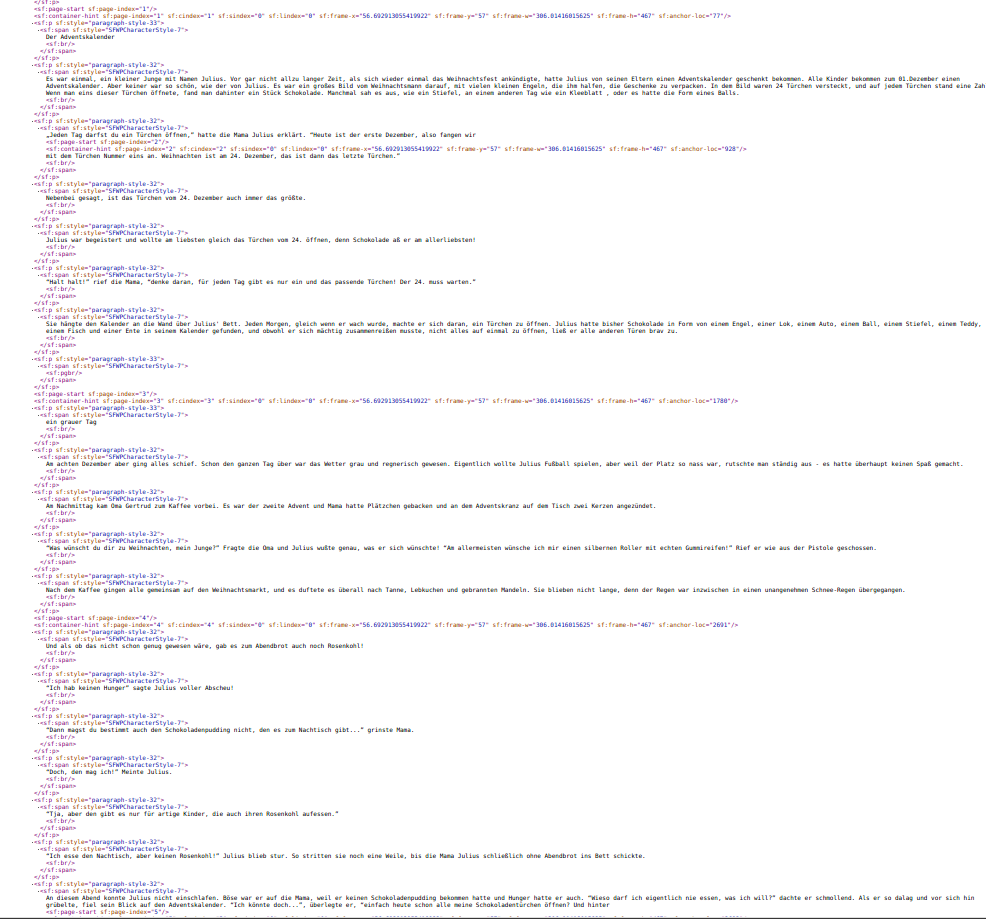
\includegraphics[height=6cm]{pics/der_eigentliche_text.png}
    \end{center}
\end{frame}

\only<article>{
  Bei der Übertragung über das Netz ist die Datei--Größe trotz ``dicker Leitungen'' nach wie vor entscheidend: Ein Word- Dokument mit dem gleichen Inhalt ist sieben mal (Word97-2003) bzw. dreimal (Word2007) grösser, als eine html-Datei gleichen Inhalts.  html ist ein Format, das sehr schlank ist und schnell übertragen werden kann. 
  }

\begin{frame}
\frametitle{2. frei verfügbares Format}
  Ein proprietäres Format wie .doc wird laufend verändert, wobei diese Veränderungen nicht dokumentiert werden. Wer das Dokument lesen will, muss die Software zum Lesen kaufen (können\ldots).

  
\includegraphics[height=3cm]{pics/pages-2011} \hfill 
\includegraphics[height=3cm]{pics/pages-2013}
\end{frame}

\only<article>{
  Webseiten sollten aber von jedem weltweit betrachtet werden können. 

  Ein weiterer Unterschied: Dokumente von Textverarbeitungen sind dafür gemacht, dass man sie leicht editieren kann. html- Dokumente dagegen sollen nach ihrer Erzeugung zunächst mal nur angezeigt, aber nicht bearbeitet werden. 

  Der Webbrowser schickt dazu eine Anfrage an den Server ``Reich mir mal die Seite /dokument.html rüber!''. Wenn die Seite vorhanden ist, gibt der Server sie heraus, sonst wird eine Fehlermeldung angezeigt. Der Webbrowserrückt die Seite raus, der Browser zeigt die Seite an - sobald man aber weiter surft, ist sie schon wieder vergessen (grundsätzlich\ldots{} Browser speichern heute Seiten in einem sogenannten Cache, damit sie beim nächsten Aufruf schneller kommen.). Bearbeiten kann man die Seite nicht. Mit speziellen Tools lässt sich der empfangene Code natürlich editieren, dann aber nur auf dem eigenen Rechner betrachten. Der Server wird es nicht erlauben, dass jeder einfach seine Änderungen auf ihm abspeichert.

  Und schliesslich gibt es für für Textverarbeitungen fest definierte Dokumentgrößen (A4 z.B.), Webseiten müssen aber auf den unterschiedlichsten Monitorgrößen angezeigt werden. Das bedeutet, dass z.B. Zeilenumbrüche flexibel sein müssen.
  }

  
\subsection{html}
\only<article>{
  html ist zunächst einmal keine Programmiersprache. Man kann keinen Rechner damit füttern und ihm das Ergebnis von $2 + 2$ entlocken. 

  html ist eine Auszeichnungssprache, die dazu dient, Inhalt zu formatieren. Dazu versieht der Programmierer den strukturierten Inhalt mit Tags --- eines zum Anfang und eines zum Ende des jeweiligen Bereichs. So kennzeichnen beispielsweise \lstinline{<p> </p>} einen Absatz. Zwischen den Tags steht dann der Inhalt.
  }

\begin{frame}{\only<presentation>{Dokumentformen}}
  \begin{itemize}
    \item Warum nicht Word, Pages, \ldots ?
    \item html
  \end{itemize}
\end{frame}
%
\begin{frame}[fragile]
\frametitle{eine einfache Seite}
  \begin{lstlisting}
    <html>
      <head>
        <title>Der Hase und der Baum</title>
      </head>
      <body>
        <h1>Der Hase und der Baum</h1>
        <h2>Kapitel 1: Der Hase</h2>
        <p>Meister Lampe hoppelt über ein Feld.</p>
        <h2>Kapitel2: In der Werkstatt</h2>
        <p>Herr K. bestellt eine Knautschzone.</p>
      </body>
    </html>
  \end{lstlisting}
\end{frame}

\begin{frame}
\frametitle{\ldots sieht so aus:}
  \begin{center}
    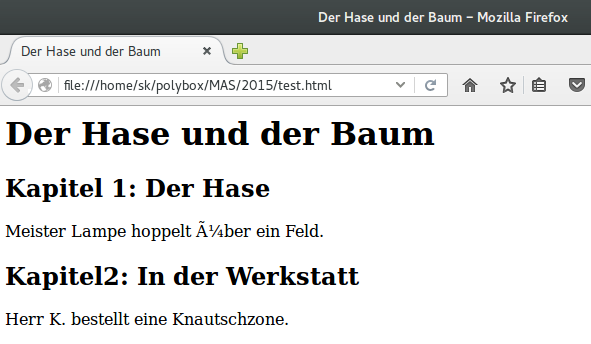
\includegraphics[width=0.8\textwidth]{pics/testseite.png}
  \end{center}
\end{frame}

\begin{frame}[fragile]
\frametitle{\ldots mit Umlauten:}
  \begin{lstlisting}
    <html>
      <head>
      <meta charset="utf-8" />
        <title>Der Hase und der Baum</title>
      </head>
      <body>
        <h1>Der Hase und der Baum</h1>
        <h2>Kapitel 1: Der Hase</h2>
        <p>Meister Lampe hoppelt über ein Feld.</p>
        <h2>Kapitel2: In der Werkstatt</h2>
        <p>Herr K. bestellt eine Knautschzone.</p>
      </body>
    </html>
  \end{lstlisting}
\end{frame}
%
\begin{frame}
\frametitle{\ldots sieht so aus:}
  \begin{center}
    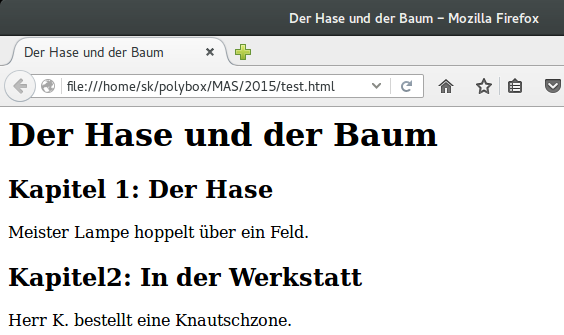
\includegraphics[width=0.8\textwidth]{pics/testseite-utf8.png}
  \end{center}
\end{frame}
%
\subsection{pdf}
\only<article>{
  Wenn man ein Dokument mit festem Layout veröffentlichen möchte, bietet sich PDF an. Es ist frei verfügbar, kann also von jedem gelesen werden, und sieht immer gleich aus. Wie auch Webseiten lässt es sich (eigentlich) nicht vom Empfänger verändern.
  }

\begin{frame}{\only<presentation>{Dokumentformen}}
  \begin{itemize}
    \item Warum nicht Word, Pages, \ldots ?
    \item html
    \item pdf
  \end{itemize}
\end{frame}
%
\begin{frame}[<+->]{Eigenschaften von pdf}
  \begin{itemize}
    \item proprietär, aber offen gelegt
    \item Papiergrösse, Layout und Inhalt festgelegt
    \item Text als Text, Bild als Bild enthalten
  \end{itemize}
\end{frame}
%
\begin{frame}{Wieder die Dokumentgrösse:}
  \begin{columns}
    \begin{column}{0.5\textwidth}
      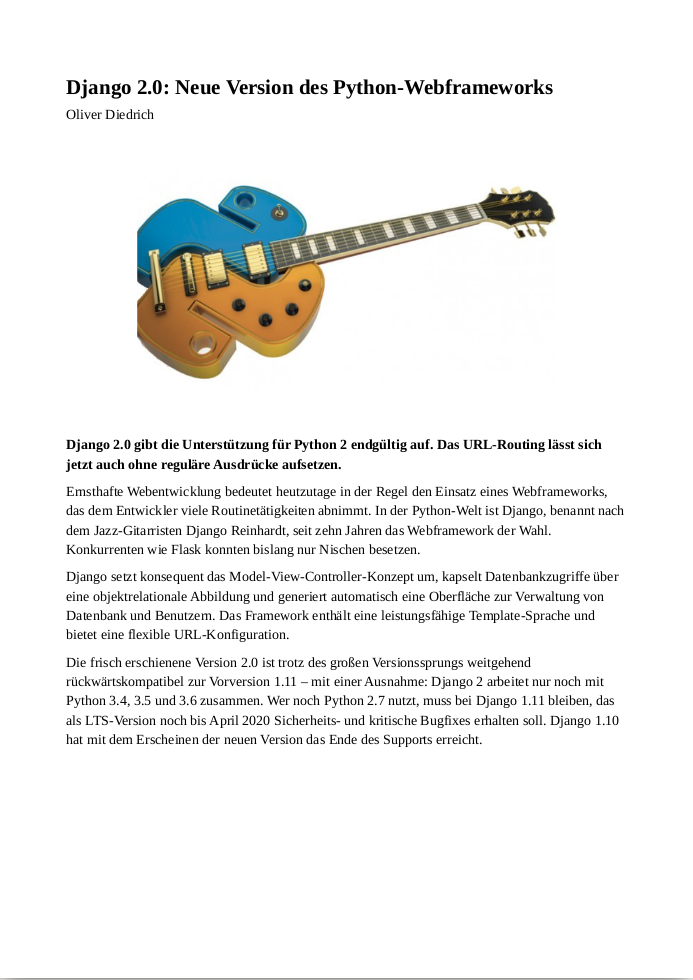
\includegraphics[width=0.9\textwidth]{pics/screenshot-beispielpdf.png}
    \end{column}
    \begin{column}{0.5\textwidth}
      als Bild: 178.8 kB\\
      als PDF: 67.7 kB
    \end{column}
  \end{columns}
\end{frame}

\begin{frame}
\frametitle{Fazit: Welche Form wofür?}
    \textbf{Textverarbeitung:} Alles zum Weiterverarbeiten

    \textbf{html:} Inhalt geht über Form

    \textbf{PDF:} Form soll erhalten bleiben
\end{frame}

\begin{frame}
\frametitle{alles Quatsch?}
\begin{theorem}
  Im Web liest doch niemand mehr. Da sollte man nur knappe Infos unterbringen.
\end{theorem}
\end{frame}

\subsection{Exkurs: stateless}
  \only<article>{
    Ein Problem bei der Entwicklung von Web--Apps war, dass ein Webserver eigentlich nichts vom User weiss. Er liefert die geforderte Webseite aus und hat dann den User schon wieder ``vergessen''.
  }
\begin{frame}
\frametitle{http is stateless}
  
\includegraphics[width=0.8\textwidth]{pics/whatsyournameagain}
\end{frame}

\begin{frame}[fragile]
  \begin{quote}
    \ldots some web applications may have to track the user's progress from page to page\ldots Solutions for these cases include:
    \begin{itemize}
      \item the use of HTTP cookies.
      \item server side sessions,
      \item hidden variables (when the current page contains a form), and
      \item URL-rewriting using URI-encoded parameters, e.g., \lstinline{/index.php?session_id=some_unique_session_code}.
    \end{itemize}
    \hfill(wikipedia)
  \end{quote}
\end{frame}

\only<article>{
  Um das zu ändern gibt es verschiedene Techniken wie z.B. Cookies und Sessions. Dabei handelt die Web--App einen eindeutigen Identifier aus und kann so wiederkehrende User identifizieren. ``Dank'' der Werbeindustrie wurden diese Techniken so weit optimiert, dass wir im Internet gläsern sind. Man kann feststellen, woher wir kommen, welche Seiten wir gesehen haben, welche wir wegklicken, wie lange wir wo verweilt haben und, und, und. 
  }

\begin{frame}
\frametitle{privacy?}
  \begin{quote}
    You have zero privacy anyway. Get over it. \hfill(Scott McNealy, Sun Microsystems, 1999)
  \end{quote}
\end{frame}

\subsection{Skriptsprachen}

\begin{frame}
  \begin{center}
    
\includegraphics[width=1\textwidth]{pics/scriptsprachen-logos}
  \end{center}
\end{frame}

\only<article>{
    Wärend man mit Auszeichnungssprachen wie z.B. html oder \LaTeX\ Dokumente formatiert, dienen Skriptsprachen wie Perl, Ruby oder Javascript dazu, einfache, wiederkehrende Aufgaben am Computer zu übernehmen.

    Beim Publishing von Aleph erhalten wir beispielsweise unzählige komprimierte Dateien, die ihrerseits unzählige XML-Dateien enthalten. Jede dieser XML-Dateien enthält einen Datensatz.
  }

\begin{frame}{Das erste Programm}
  \begin{center}
    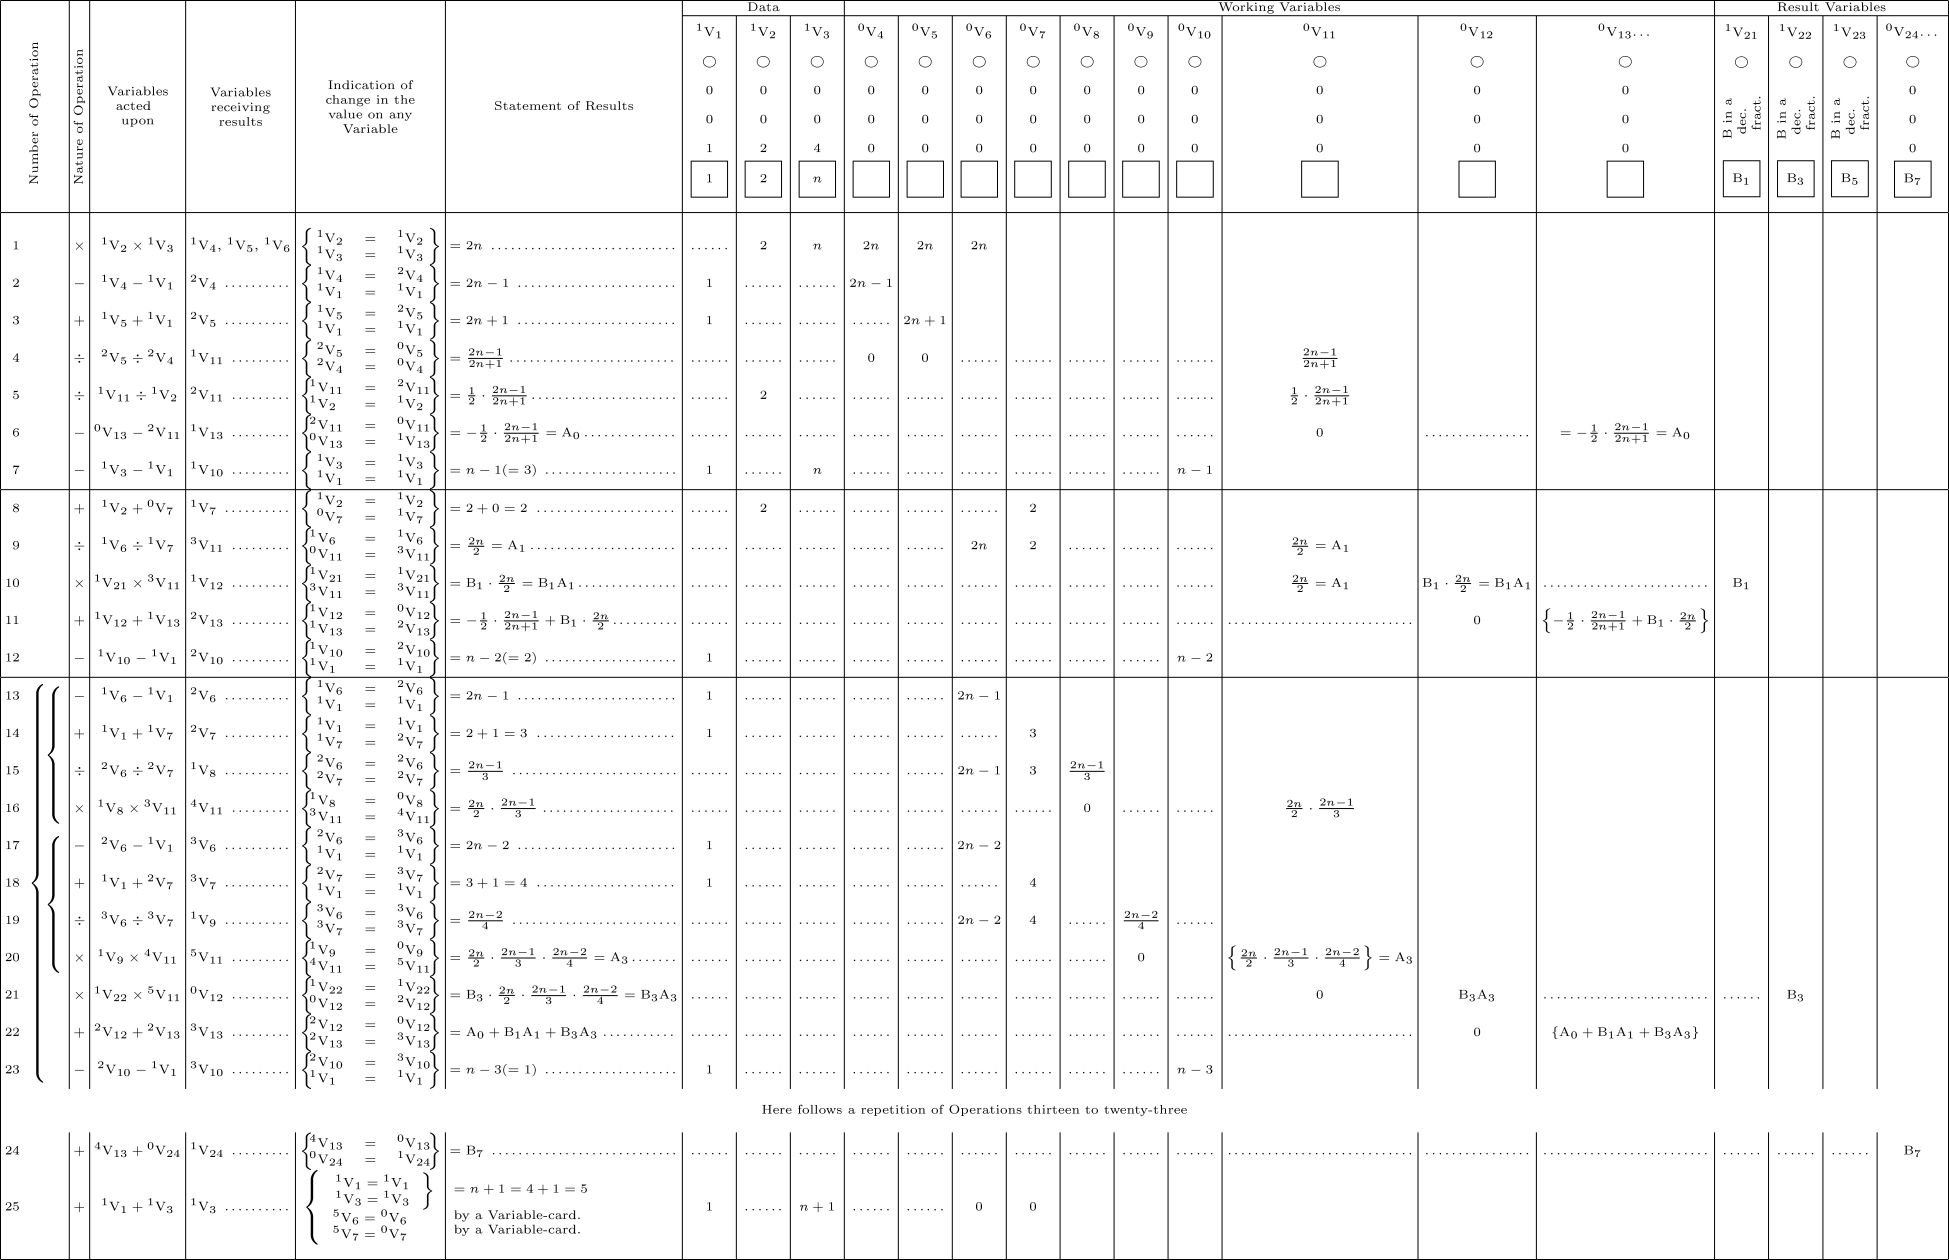
\includegraphics[width=0.8\textwidth]{pics/dasersteprogramm.png}
  \end{center}
\end{frame}

\begin{frame}{Spielereien in Perl und Ruby}
  Die Aufgabe lautet, ein Programm zu schreiben, das die Zahlen von 1 -- 100 hoch zählt und 
  \begin{itemize}
    \item bei Zahlen, die durch \textbf{drei} teilbar sind, ,,Fizz'' ausgibt,
    \item bei Zahlen, die durch \textbf{fünf} teilbar sind, ,,Buzz'' ausgib und
    \item bei Zahlen, die durch \textbf{beides} teilbar sind, ,,FizzBuzz'' ausgibt.
  \end{itemize}
\end{frame}

\begin{frame}{Ansatz in Perl}
  \begin{center}
    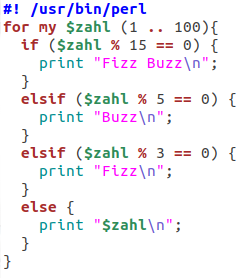
\includegraphics[height=0.6\textheight]{pics/fizzbuzz-perl.png}
  \end{center}
\end{frame}
%
\begin{frame}{Ansatz in Ruby}
  \begin{center}
    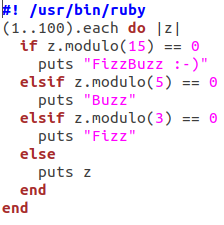
\includegraphics[height=0.6\textheight]{pics/fizzbuzz-ruby.png}
  \end{center}
\end{frame}

\begin{frame}{Ein Programm}
  Das folgende Ruby--Skript (Auszug) dient zum Durchsuchen von tar-files:
  
  \begin{center}
    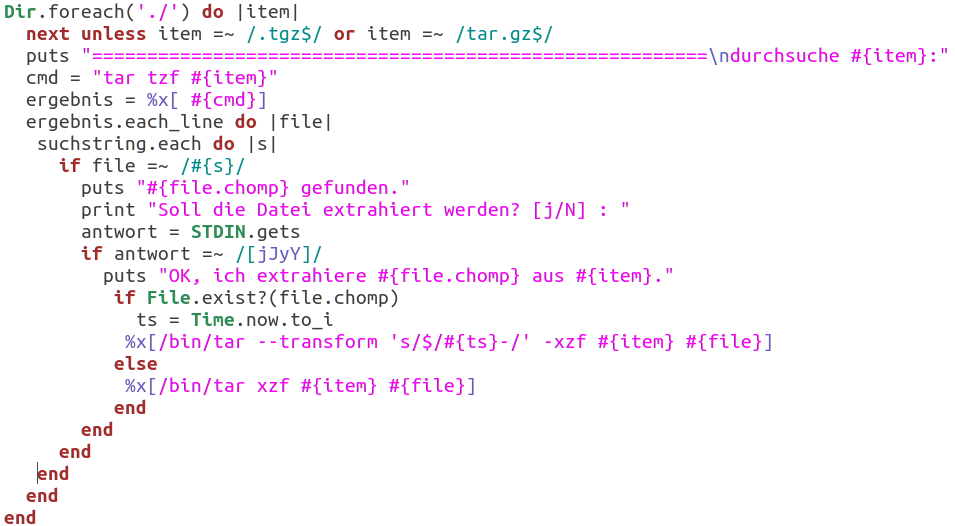
\includegraphics[height=0.7\textheight]{pics/tarsearch-ruby.png}
  \end{center}
\end{frame}

\subsection{Ajax}
\begin{frame}{Ajax}
  Interaktion mit dem User durch:
  \begin{center}
    \textbf{A}synchronous \textbf{J}avaScript \textbf{A}nd \textbf{X}ML
  \end{center}
\end{frame}

\only<presentation>{
\begin{frame}{Wo wird was ausgeführt?}
  ?
\end{frame}
}

%
\begin{frame}{dynamische Webseiten}
\framesubtitle{Was kann wo manipuliert werden?}
  \begin{center}
    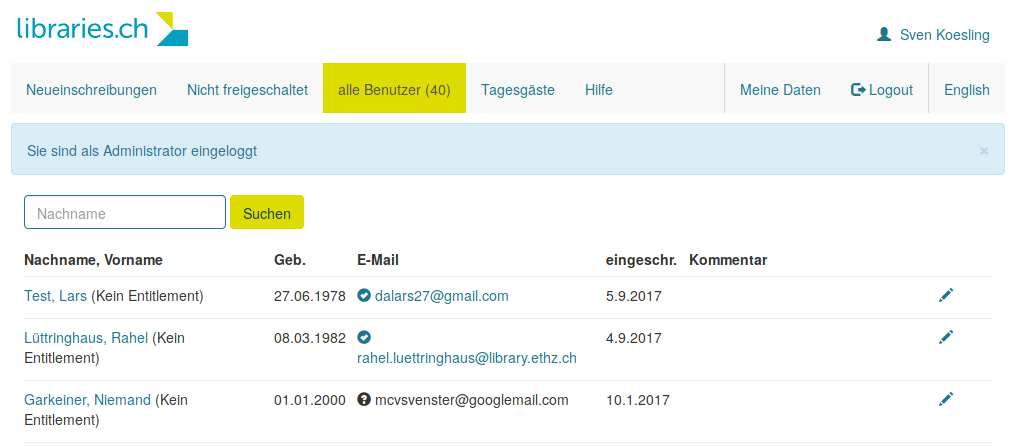
\includegraphics[height=0.7\textheight]{pics/ajax-pidp.png}
  \end{center}
\end{frame}

\begin{frame}{}
\framesubtitle{Elemente einer Webseite im Quelltext}
  ein Benutzer mit verifizierter EMail--Adresse:

  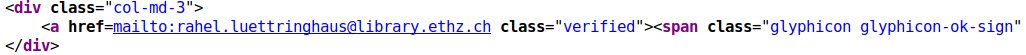
\includegraphics[width=1\textwidth]{pics/class-verified.png}
  \ldots und einer mit einer unbekannten EMail--Adresse:
  
  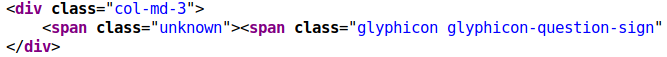
\includegraphics[width=0.7\textwidth]{pics/class-unknown.png}
\end{frame}


\subsection{Responsive Web}
\begin{frame}{\only<presentation>{Responsive Web}}
\framesubtitle{So soll es nicht sein!}
  \begin{center}
    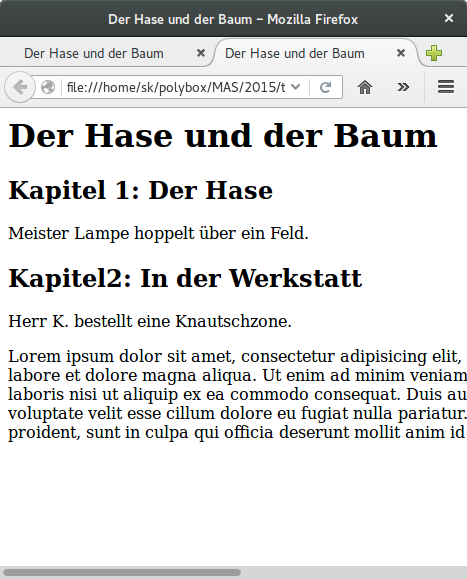
\includegraphics[width=0.4\textwidth]{pics/testseite-feste_breite.png}
  \end{center}
\end{frame}
%
\begin{frame}
\frametitle{So soll es sein:}
  \begin{center}
    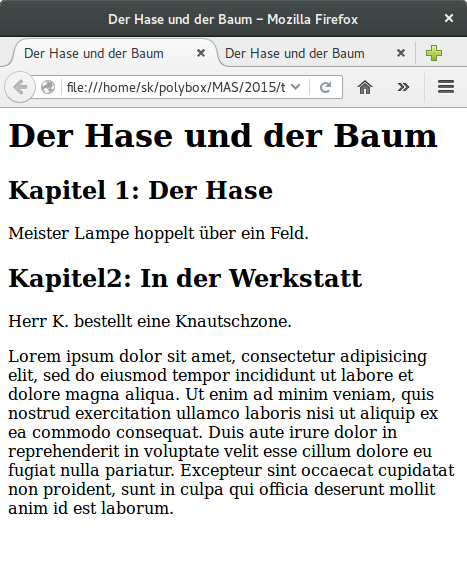
\includegraphics[width=0.4\textwidth]{pics/testseite-gut.png}
  \end{center}
\end{frame}
%

\section{Datenbanktechnologien I}
%
\begin{frame}[<+->]{Warum Datenbanken?}
  \begin{itemize}
    \pause
    \item geringer Speicherplatzbedarf
    \item gleichzeitiger Zugriff durch viele Nutzer
  \end{itemize}
\end{frame}

\only<article>{
  Da Speicher früher sehr teuer war, entwickelte man Strategien, um Speicherplatz zu sparen. Ein gutes Beispiel sind Normalisierungen bei relationalen Datenbanken.
  }

\subsection{Datenbanktypen}
\begin{frame}[<+->]{Welche Typen von Datenbanken gibt es?}
  \begin{itemize}
    \pause
    \item K/V-- Stores
    \item relationale Datenbanken
    \item Spaltenorientierte Datenbanken
    \item Dokumentorientierte Datenbanken
    \item Graphendatenbanken
  \end{itemize}
\end{frame}

\subsection*{K/V-- Stores}

\begin{frame}{\only<presentation>{K/V-- Stores}}
  K/V-- Stores sind --- wie der Name schon sagt --- schlichte Schlüssel / Wert-- Speicher. Sie sind bei minimalem Speicherplatzbedarf sehr schnell, was sie für das Caching von Werten prädestiniert.
\end{frame}

\subsection*{relationale Datenbanken}
\only<article>{
  Nehmen wir zur Verdeutlichung eine Versicherung, die die Adressen ihrer Kunden in einer Datenbank speichern möchte. Es wird eine grosse Tabelle angelegt, je eine Zeile pro Kunde. Dabei stellt sich heraus, dass die Versicherung 1000 Kunden hat, die in der Hauptstrasse wohnen. Das bedeutet, dass wir 1000 Mal den Speicherplatz für das Wort ``Hauptstrasse'' benötigen.}
      
\begin{frame}{relationale Datenbanken}
\framesubtitle{Eine Kundentabelle}
  \begin{center}
    \begin{tabular}{lllll}
      id & Nachname & Vorname & Strasse & Stadt\\
      \hline
      1 & Muster & Hans & Hauptstrasse & Zürich\\
      2 & Meier & Heinrich & Hauptstrasse & Zürich\\
      3 & Müller & Hubert & Hauptstrasse & Zürich\\
      4 & Schulze & Herbert & Hauptstrasse & Zürich\\
    \end{tabular}
  \end{center}
\end{frame}

\only<article>{
  Wenn man nun die Strassen in eine extra Tabelle schreibt, eine Zeile pro Strasse, dann muss man in der Tabelle der Kunden nur die ID der Strasse hinterlegen. Wenn die Hauptstrasse z.B. die ID 1 hat, dann benötigen wir nur noch 1000 Mail den Speicherplatz für den Integer 1 --- wesentlich weniger, als für den String ``Hauptstrasse''. Analog kann man z.B. auch mit Städten verfahren. 
        }

\begin{frame}{relationale Datenbanken}
\framesubtitle{Tabelle der Strassen}
  \begin{center}
    \begin{tabular}{ll}
      id & Strasse\\
      \hline
      1 & Hauptstrasse\\
      2 & Nebenstrasse\\
      3 & Seitenstrasse\\
    \end{tabular}
  \end{center}
\end{frame}
%
\begin{frame}{relationale Datenbanken}
\framesubtitle{Tabelle der Städte}
  \begin{center}
    \begin{tabular}{ll}
      id & Stadt\\
      \hline
      1 & Zürich\\
      2 & Basel\\
      3 & Bern\\
    \end{tabular}
  \end{center}
\end{frame}

\begin{frame}{relationale Datenbanken}
\framesubtitle{Tabelle mit Relationen}
  \begin{center}
    \begin{tabular}{lllcc}
      id & Nachname & Vorname & Strassen\_ID & Stadt\_ID\\
      \hline
      1 & Muster & Hans & 1 & 1\\
      2 & Meier & Heinrich & 1 & 1\\
      3 & Müller & Hubert & 1 & 1\\
      4 & Schulze & Herbert & 1 & 1\\
    \end{tabular}
  \end{center}
\end{frame}
%
\begin{frame}{relationale Datenbanken}
\framesubtitle{Normalisierung}
  Eine relationale Datenbank dahingehend zu optimieren, dass es möglichst wenig Redundanzen gibt, nennt man ,,normalisieren''. Es gibt fünf Normalformen.
\end{frame}
%
\begin{frame}{relationale Datenbanken}
\framesubtitle{Normalisierung: Speicherplatzbedarf}
  \begin{center}
    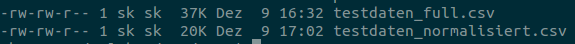
\includegraphics[width=0.8\textwidth]{pics/speicherplatzbedarf}
  \end{center}
\end{frame}
      
\only<article>{
  Für die Datenbank--Spezialisten war es eine komplexe Aufgabe, Daten optimal zu normalisieren.
      
  Die Normalisierung hat auch Nachteile. So liegen nicht alle Informationen in einer Tabelle, was Abfragen komplexer macht. Damit einher geht ein höherer Leistungsbedarf des Servers.
  }

\begin{frame}{relationale Datenbanken}
\framesubtitle<presentation>{Relationen in der DB von Aleph}
  \begin{figure}
    \begin{center}
      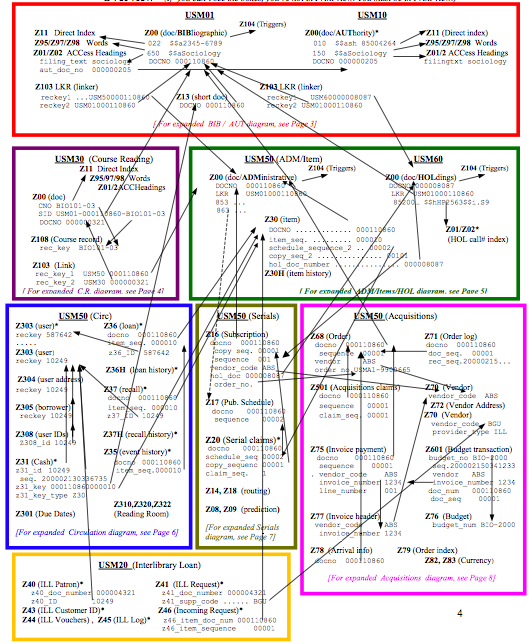
\includegraphics[width=0.4\textwidth]{pics/alephtables}
        \only<article>{\caption{Relationen in der DB von Aleph}}
      \end{center}
    \end{figure}
\end{frame}

\begin{frame}[fragile]{relationale Datenbanken}
\framesubtitle{Felder nicht atomar}
  \begin{lstlisting}
    select substr(z103_rec_key,6,9) || 'EHO60'
      from eho60.z103
      where substr(z103_lkr_text_n,1,3) = 'E04'
      and z103_lkr_library = 'EBI01'
      and substr(z103_rec_key,1,5) = 'EHO60'
    ;
  \end{lstlisting}
\end{frame}
        
\only<article>{
  Ein Nachteil von relationalen Datenbanken ist die feste Grösse und Anzahl von Feldern. Wenn ich beispielsweise für die Tabelle der Kunden die Spalten
      
  \begin{tabular}{rrrrrr}
    Vorname & Nachname & Strasse & Hausnummer & Postleitzahl & Ort\\
  \end{tabular}
      
  festgelegt habe, und die Versicherung sich entscheidet, ein internationales Geschäft aufzubauen, ist es einiger Aufwand, die Spalte ``Land'' hinzu zu fügen.
  }

\begin{frame}{relationale Datenbanken}
\framesubtitle{feste Feldgrösse}
  Das Feld für Inventarnummern darf in Aleph nicht mehr als 20 Zeichen haben. 
\end{frame}
%
\begin{frame}{relationale Datenbanken}
\framesubtitle{und wieder: Kodierung von Text}
  \begin{quote}
    UTF8-Codierungszeichen zaehlen einzeln, auch wenn daraus ein einziges Unicode-Zeichen entsteht. 

    Ein Beispiel dafuer ist das ``Ä'', das im Inventarnummernfeld zwei VARCHAR2 Zeichen aufbraucht, weil es aus 0xc3 und 0x84 besteht. 

    Ich habe nicht geschaut, ob es noch weitere solche Fälle gibt. \hfill{[Mathias Weyland]}
  \end{quote}
\end{frame}
%
\begin{frame}{relationale Datenbanken}
\framesubtitle{Quasi--Monopole}
  \begin{figure}
    \begin{center}
      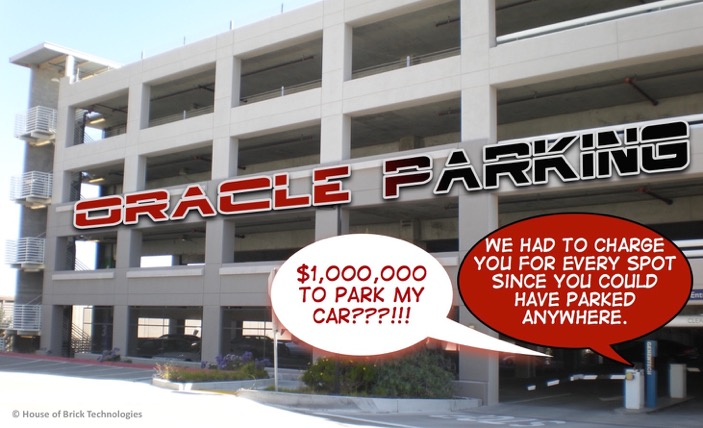
\includegraphics[width=0.8\textwidth]{pics/Oracle-Parking}
      \end{center}
      \caption{http://houseofbrick.com/the-oracle-parking-garage/}
    \end{figure}
\end{frame}
%
\subsection{dokumentorientierte Datenbanken}
\begin{frame}
  \frametitle<beamer>{dokumentorientierte Datenbanken}
  \begin{center}
    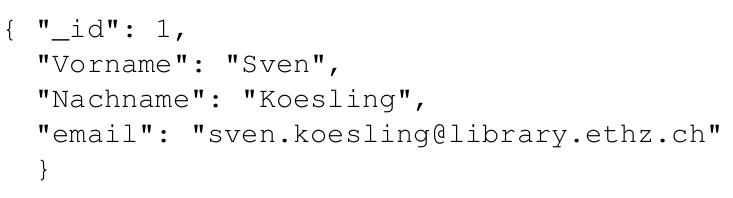
\includegraphics[width=0.8\textwidth]{pics/doc1}
  \end{center}
\end{frame}

\begin{frame}{ein weiteres Dokument in derselben collection}
  \begin{center}
  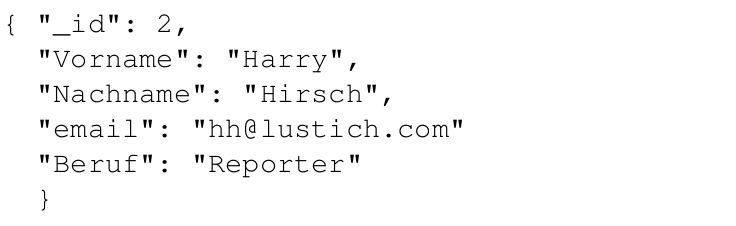
\includegraphics[width=0.8\textwidth]{pics/doc2}
  \end{center}
\end{frame}
     
\begin{frame}
  \frametitle{noch ein Dokument in derselben collection}
  \begin{center}
  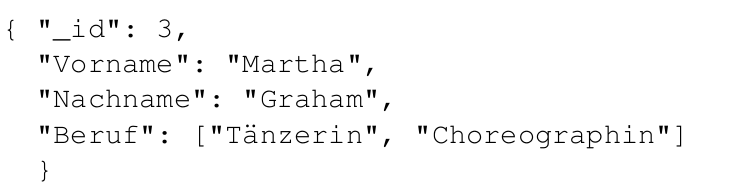
\includegraphics[width=0.8\textwidth]{pics/doc3}
  \end{center}
\end{frame}

\begin{frame}{und noch ein weiteres Dokument in derselben collection}
  \begin{center}
    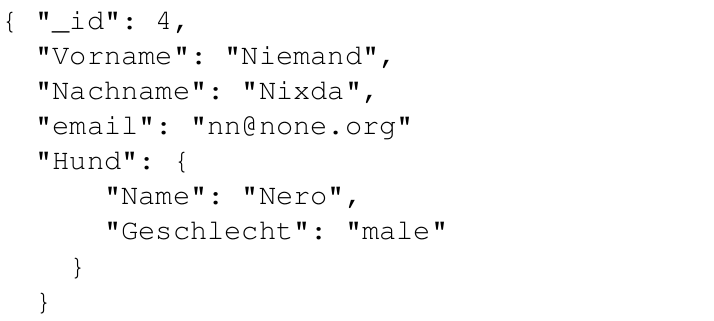
\includegraphics[width=0.8\textwidth]{pics/doc4}
  \end{center}
\end{frame}

\only<article>{
  Wenn wir an Dokumente denken, kommen wir schnell auf die ,,Panama--Papers''. 
  }
\subsection*{Graphendatenbanken}

\begin{frame}{\only<presentation>{Graphendatenbanken}}
  Graphendatenbanken sind quasi Knoten und Kanten mit Attributen.
\end{frame}

\begin{frame}{ein paar Knoten}
  \begin{center}
    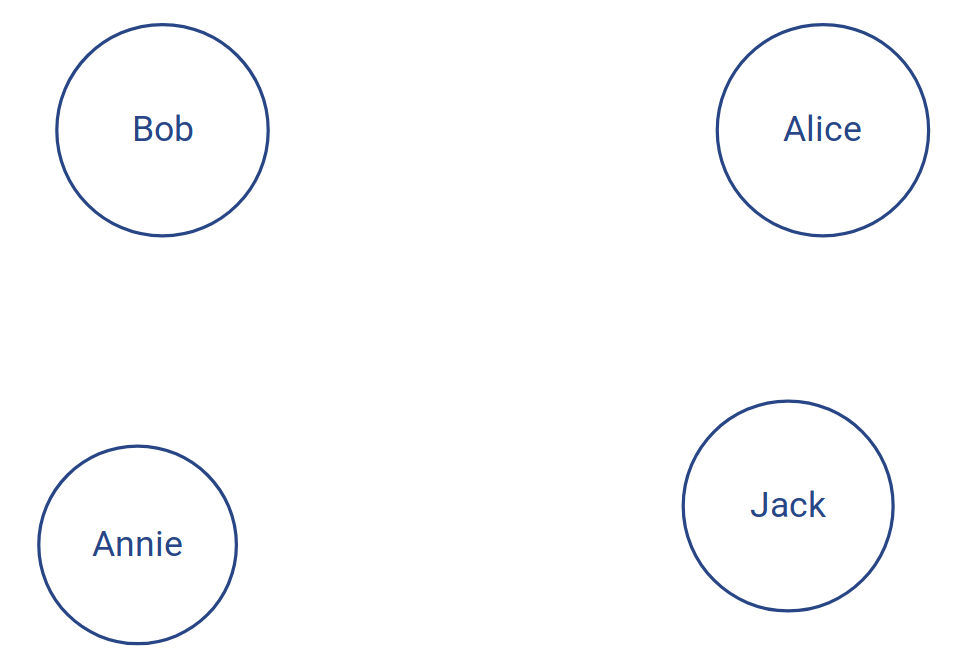
\includegraphics[width=0.8\textwidth]{pics/knoten}
  \end{center}
\end{frame}

\begin{frame}{Knoten und Beziehungen}
  \begin{center}
    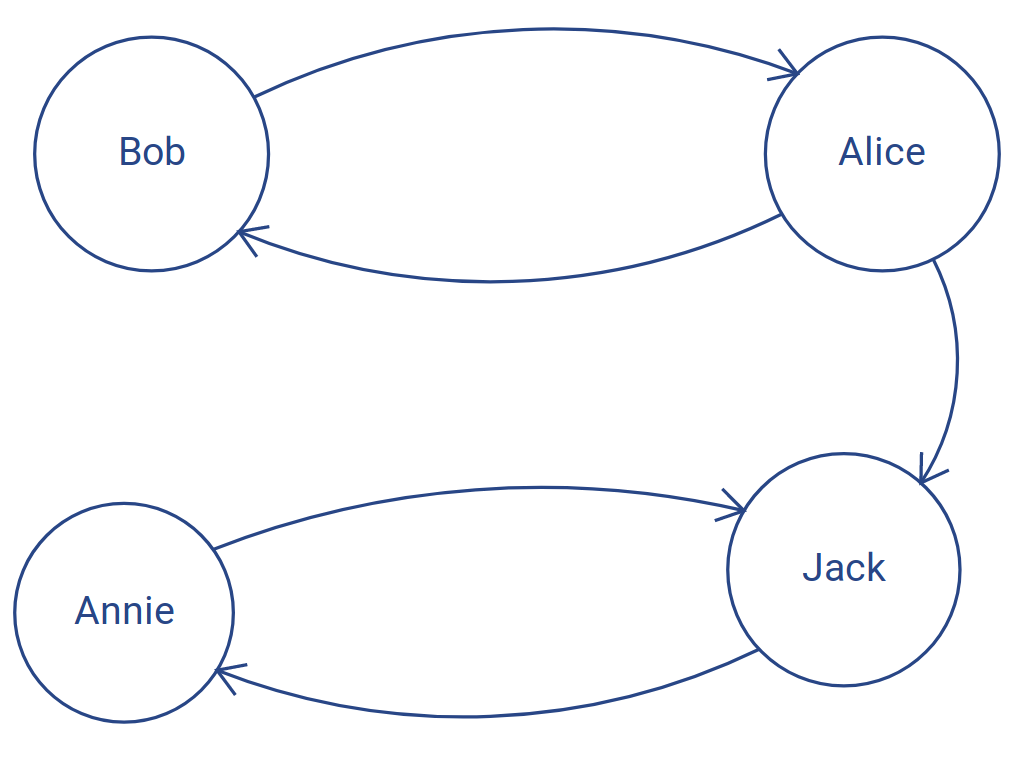
\includegraphics[width=0.8\textwidth]{pics/knoten-beziehungen}
  \end{center}
\end{frame}

\begin{frame}{Knoten, Beziehungen und Attribute}
  \begin{center}
    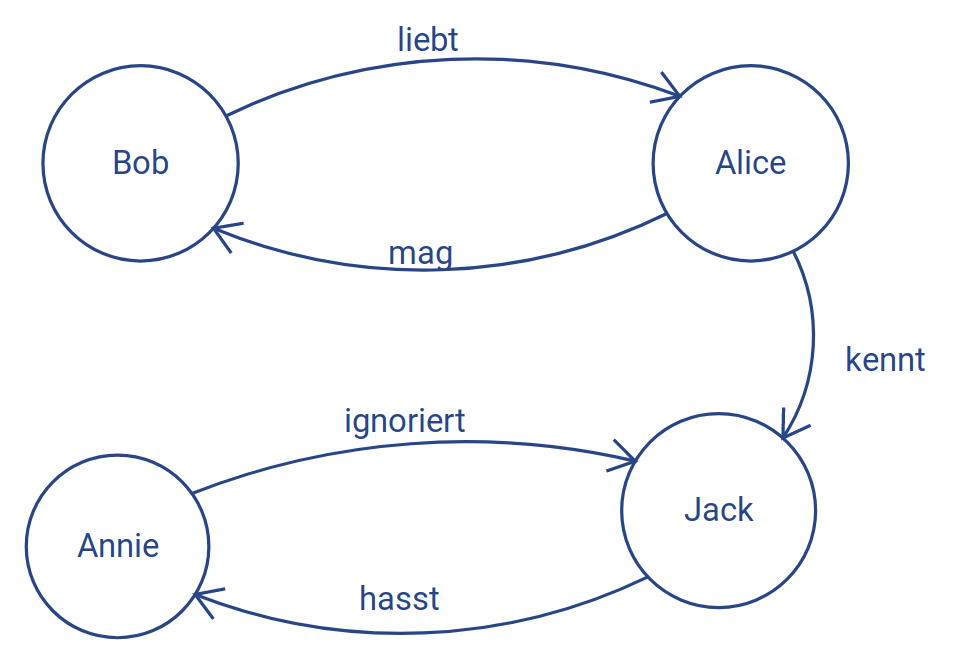
\includegraphics[width=0.8\textwidth]{pics/knoten-beziehungen-attribute}
  \end{center}
\end{frame}

\subsection{Exkurs: Indexer}
\begin{frame}{}
  \begin{figure}
    \caption{Suche nach ``Landquart'' in einem aktuellen Bibliothekskatalog (420.000 Dokumente): 1072 Treffer -- ohne Facetten: completed in 2845ms}
    \begin{center}
      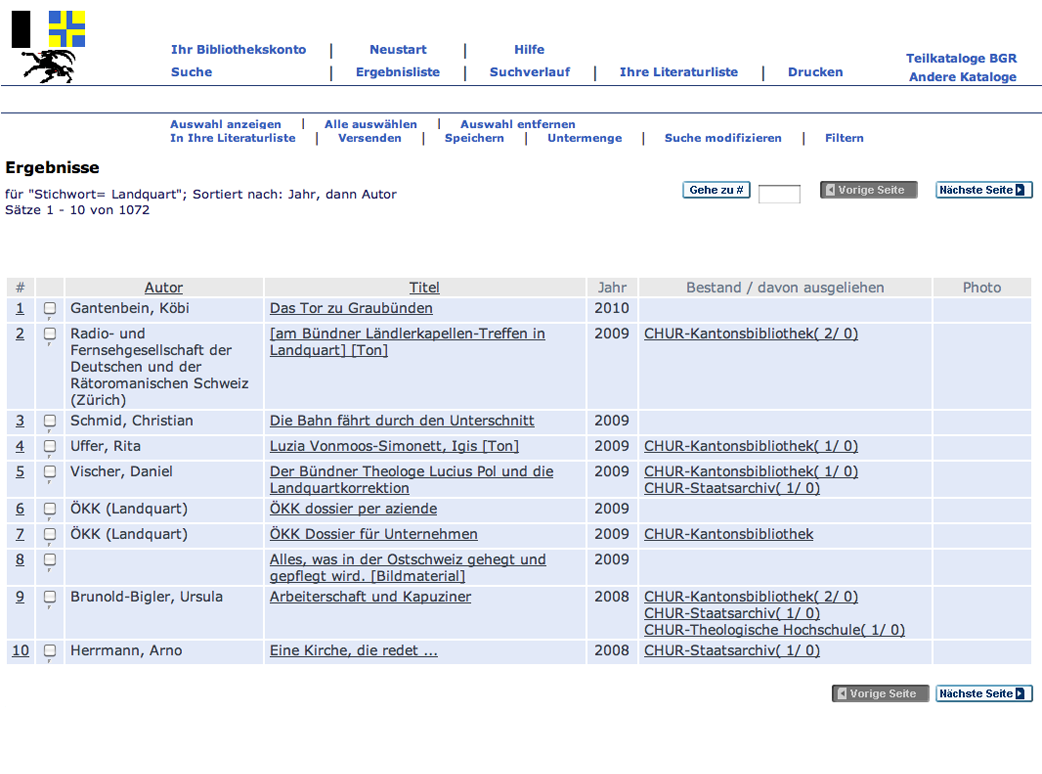
\includegraphics[width=0.8\textwidth]{pics/aleph}
    \end{center}
  \end{figure}
\end{frame}

\begin{frame}
  \begin{figure}
    \caption{Die gleiche Suche mit einem Indexer: 1.700 Treffer mit drei Facetten: completed in 792ms}
    \begin{center}
      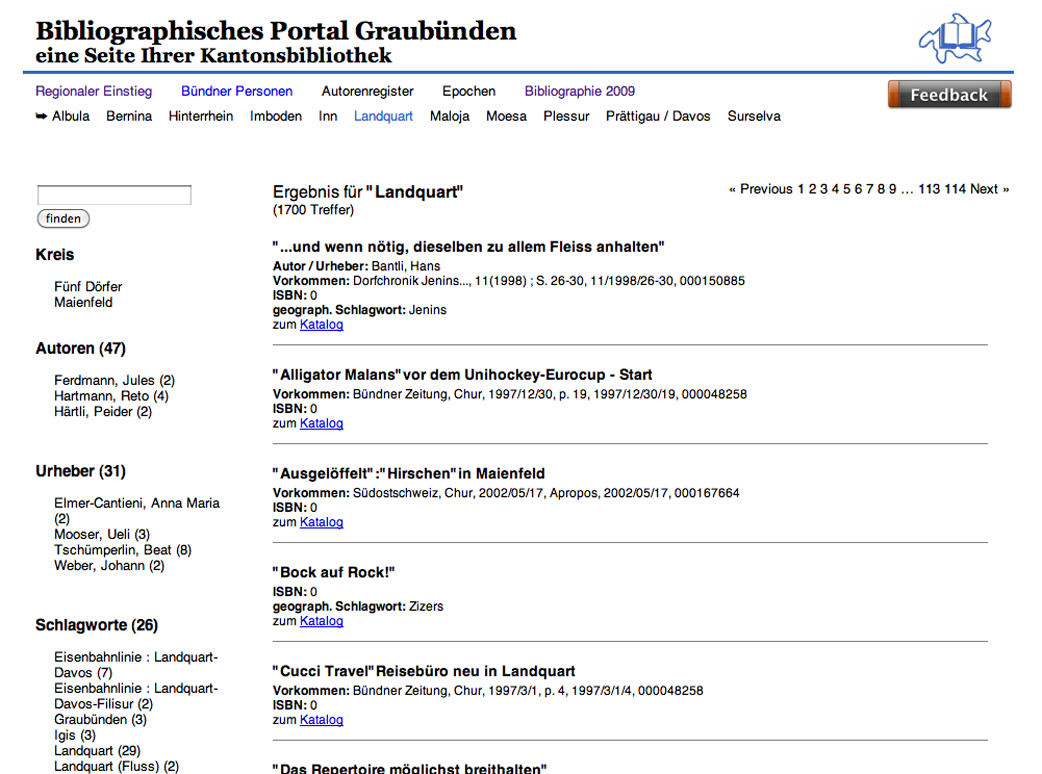
\includegraphics[width=0.8\textwidth]{pics/Ergebnis}
    \end{center}
  \end{figure}
\end{frame}}
